% \iffalse
\let\negmedspace\undefined
\let\negthickspace\undefined
\documentclass[journal,12pt,twocolumn]{IEEEtran}
\usepackage{cite}
\usepackage{amsmath,enumitem,amssymb,amsfonts,amsthm}
\usepackage{algorithmic}
\usepackage{graphicx}
\usepackage{float}
\usepackage{textcomp}
\usepackage{xcolor}
\usepackage{caption}
\usepackage{txfonts}
\usepackage{listings}
\usepackage{enumitem}
\usepackage{mathtools}
\usepackage{gensymb}
\usepackage{comment}
\usepackage[breaklinks=true]{hyperref}
\usepackage{tkz-euclide} 
\usepackage{listings}
\usepackage{tabularx}
\usepackage{gvv}                                        
\def\inputGnumericTable{}                                 
\usepackage[latin1]{inputenc}                              
\usepackage{color}                                            
\usepackage{array}                                            
\usepackage{longtable}                                       
\usepackage{calc}                                             
\usepackage{multirow}                                         
\usepackage{hhline}                                           
\usepackage{ifthen}                                        
\usepackage{lscape}
\newtheorem{theorem}{Theorem}[section]
\newtheorem{problem}{Problem}
\newtheorem{proposition}{Proposition}[section]
\newtheorem{lemma}{Lemma}[section]
\newtheorem{corollary}[theorem]{Corollary}
\newtheorem{example}{Example}[section]
\newtheorem{definition}[problem]{Definition}
\newcommand{\BEQA}{\begin{eqnarray}}
\newcommand{\EEQA}{\end{eqnarray}}
\newcommand{\define}{\stackrel{\triangle}{=}}
\theoremstyle{remark}
\newtheorem{rem}{Remark}
\begin{document}



\bibliographystyle{IEEEtran}
\vspace{3cm}

\title{NCERT 11.9.5 26Q}
\author{EE23BTECH11015 - DHANUSH V NAYAK$^{*}$% <-this % stops a space
}
\maketitle
\newpage
\bigskip

\renewcommand{\thefigure}{\arabic{figure}}
\renewcommand{\thetable}{\theenumi}

\bibliographystyle{IEEEtran}
\textbf{Question:}
\begin{align}
    \frac{1\times2^2 + 2\times3^2 + \dots + n\times\brak{n+1}^{2}}{1^2\times2 + 2^2\times3 + \dots + n^2\times \brak{n+1}}\notag 
\end{align}

Find the z-transform of general term of numerator and denominator and plot them . Also find z-transform of sum of terms of numerator and denominator and plot it.\\ 
\textbf{Solution:}

\begin{table}[h]
\centering
\renewcommand\thetable{1}
\setlength{\extrarowheight}{9pt}
\resizebox{0.54\textwidth}{!}{
\begin{tabular}{|c|c|c|}
\hline
\textbf{Parameter} & \textbf{Description} & \textbf{Value} \\ \hline
$n$ & Integer & 1, 2, 3, 4, ... \\ \hline
$x_1(n)$ & General term of Numerator & $\vphantom{\brak{n^{3}}} \brak{n^{3} + 5n^{2} + 20n + 4} \cdot u\brak{n}$ \\ \hline
$x_2(n)$ & General Term of Denominator  & $\vphantom{\brak{n^{3}}} \brak{n^{3}+4n^{2}+5n+2}\cdot u\brak{n}$ \\ \hline
$y_1\brak{n}$ & Sum of terms of numerator & $\frac{3n^4 + 26n^3 + 81n^2 + 106n + 48}{12}$ \\ \hline
$y_2\brak{n}$ & Sum of terms of denominator & $ \frac{3n^4 + 22n^3 + 57n^2 + 62n + 24}{12}$ \\ \hline
$U(z)$ & z-transform of $u(n)$ & $\frac{1}{1 - z^{-1}\vphantom {\brak{0.3pt}}},\cbrak{z\in\mathbb{C} : \lvert z \rvert > 1}$ \\ \hline 
ROC & Region of convergence & $\left\{ z : \left|\sum_{n=-\infty}^{\infty} x(n)z^{-n}\right| < \infty \vphantom {\brak{{0.3pt}}}\right\}$ \\ \hline 
\end{tabular}}
\caption{Parameter Table}
\label{tab:11.9.5.26.1}
\end{table}




\begin{enumerate}[label=\arabic*.]
\item General term of Numerator of the LHS part:
\begin{align}
    x_1\brak{n} &= \brak{n+1}\brak{n+2}^{2}\cdot u\brak{n} \\
                &= \brak{n^{3} + 5n^{2} + 20n + 4} \cdot u\brak{n}\label{eq:11.9.5.26.1} 
\end{align}
By the differentiation property :
\begin{align}
x\brak{n} &\system{Z} X\brak{z},\hspace{4pt} ROC = R\\
n^k x\brak{n} &\system{Z} \brak{-z}^k \frac{d^kX\brak{z}}{dz^k},\hspace{4pt} ROC = R \\
\implies n^k u\brak{n} & \system{Z} \brak{-z}^k \frac{d^kU\brak{z}}{dz^k} \cbrak{z\in\mathbb{C} : \lvert z \rvert > 1}
\end{align}

\begin{align}
    n\cdot u\brak{n} & \system{Z} \frac{z^{-1}}{\brak{1-z^{-1}}^2} ,\cbrak{z\in\mathbb{C} : \lvert z \rvert > 1} \\
     n^2\cdot u\brak{n} & \system{Z} \frac{z^{-1}\brak{z^{-1}+1}}{\brak{1-z^{-1}}^3} ,\cbrak{z\in\mathbb{C} : \lvert z \rvert > 1} \\
     n^3\cdot u\brak{n} & \system{Z} \frac{z^{-1}\brak{1+4z^{-1}+z^{-2}}}{\brak{1-z^{-1}}^4} ,\cbrak{z\in\mathbb{C} : \lvert z \rvert > 1} \\
    n^4\cdot u\brak{n} & \system{Z} \frac{z^{-1}\brak{1+11z^{-1}+11z^{-2}+z^{-3}}}{\brak{1-z^{-1}}^5}\\ &  \hspace{2cm}\text{where} \cbrak{z\in\mathbb{C} :\lvert z \rvert > 1} \notag 
\end{align}
\begin{align}
 X_1\brak{z} &= \sum_{n=-\infty}^\infty x_1\brak{n}\cdot u\brak{n}\cdot z^{-n}\\
             &= \sum_{n=-\infty}^\infty \brak{n^{3} + 5n^{2} + 20n + 4}\cdot u\brak{n}\cdot z^{-n}\\
 \therefore   X_1\brak{z}&= \frac{4+14z^{-1}-24z^{-2}+12z^{-3}}{\brak{1-z^{-1}}^4} ,\cbrak{z\in\mathbb{C} : \lvert z \rvert > 1} 
\end{align}
\begin{align}
y_1\brak{n}&=1\times2^2 + 2\times3^2 + \dots + n\times\brak{n+1}^2 \\
y_1\brak{n} &= \sum_{k=0}^n \brak{k+1}\brak{k+2}^2\cdot u\brak{n} \\
y_1\brak{n} &= x_1\brak{n}\ast u\brak{n}\\
    Y_1\brak{z} &= X_1\brak{z}\cdot U\brak{z} \\
 &= \frac{4+14z^{-1}-24z^{-2}+12z^{-3}}{\brak{1-z^{-1}}^5} ,\cbrak{z\in\mathbb{C} : \lvert z \rvert > 1} 
\end{align}
Using partial fractions:
\begin{align}
    Y_1(z) &= \frac{34z^{-1}}{\brak{1-z^{-1}}} + \frac{72z^{-2}}{\brak{1-z^{-1}}^2} + \frac{64z^{-3}}{\brak{1-z^{-3}}^3} \\
    &+ \frac{28z^{-4}}{\brak{1-z^{-1}}^4}+\frac{6z^{-5}}{\brak{1-z^{-1}}^5}+4 \notag \\
    Y_1(z) &= \frac{z^{-1}\brak{1+11z^{-1}+11z^{-2}+z^{-3}}}{4\cdot \brak{1-z^{-1}}^5} \\ &+ \frac{26\cdot z^{-1}\brak{1+4z^{-1}+z^{-2}}}{12\brak{1-z^{-1}}^4} 
    + \frac{27\cdot z^{-1}\brak{z^{-1}+1}}{4\brak{1-z^{-1}}^3} \notag \\ &+\frac{53\cdot z^{-1}}{6\brak{1-z^{-1}}^2} \notag 
    + 4 \frac{1}{\brak{1-z^{-1}}} \notag
\end{align}

Taking the inverse z-transform of each term : 
\begin{align}
    y_1\brak{n} &= \frac{3n^4 + 26n^3 + 81n^2 + 106n + 48}{12}
\end{align}
\item General term of Denominator of the RHS part:
\begin{align}
    x_2\brak{n} &= \brak{n+1}^{2}\brak{n+2}\cdot u\brak{n}\\
                &= \brak{n^{3}+4n^{2}+5n+2}\cdot u\brak{n} \label{eq:11.9.5.26.3}
\end{align}


\begin{align}
    X_2\brak{z} &= \sum_{n=-\infty}^\infty x_2\brak{n}\cdot u\brak{n}\cdot z^{-n}\\
                &= \sum_{n=-\infty}^\infty \brak{n^{3}+4n^{2}+5n+2}\cdot u\brak{n}\cdot z^{-n}\\
   \therefore  X_2\brak{z} &= \frac{2+4z^{-1}}{\brak{1-z^{-1}}^4},\cbrak{z\in\mathbb{C} : \lvert z \rvert > 1}   
\end{align}
\begin{align}
    y_2\brak{n} &= 1^2\times2 + 2^2\times3 + \dots + n^2\times\brak{n+1}\\
    y_2\brak{n} &= \sum_{k=0}^n \brak{k+1}^2\brak{k+2}\cdot u\brak{n} \\
    y_2\brak{n} &= x_2\brak{n}\ast u\brak{n}\\
    Y_2\brak{z} &= X_2\brak{z}\cdot U\brak{z} \\
 &=\frac{2+4z^{-1}}{\brak{1-z^{-1}}^5} ,\cbrak{z\in\mathbb{C} : \lvert z \rvert > 1} 
\end{align}
Using partial fractions:
\begin{align}
    Y_2\brak{z} &= \frac{14z^{-1}}{\brak{1-z^{-1}}} + \frac{36z^{-2}}{\brak{1-z^{-1}}^2} + \frac{44z^{-3}}{\brak{1-z^{-3}}^3} \\&+ \frac{26z^{-4}}{\brak{1-z^{-1}}^4}+\frac{6z^{-5}}{\brak{1-z^{-1}}^5}+2\notag \\
     Y_2(z) &= \frac{z^{-1}\brak{1+11z^{-1}+11z^{-2}+z^{-3}}}{4\cdot \brak{1-z^{-1}}^5} \\ &+ \frac{11\cdot z^{-1}\brak{1+4z^{-1}+z^{-2}}}{6\brak{1-z^{-1}}^4} 
    + \frac{19\cdot z^{-1}\brak{z^{-1}+1}}{4\brak{1-z^{-1}}^3} \notag \\ &+\frac{31\cdot z^{-1}}{6\brak{1-z^{-1}}^2} \notag 
    + 2\frac{1}{\brak{1-z^{-1}}} \notag
\end{align}
Taking the inverse z-transform of each term:
\begin{align}
    y_2\brak{n} =  \frac{3n^4 + 22n^3 + 57n^2 + 62n + 24}{12}
\end{align}
\end{enumerate}

\begin{figure}[htbp]
    \centering
    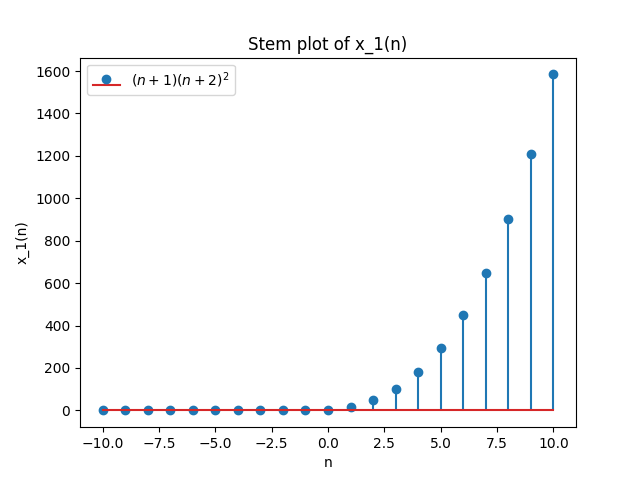
\includegraphics[width=1\columnwidth]{x1_plot.png}
    \caption{Stem Plot of $x_1\brak{n}$}
    \label{fig:x1}
\end{figure}

\begin{figure}[htbp]
    \centering
    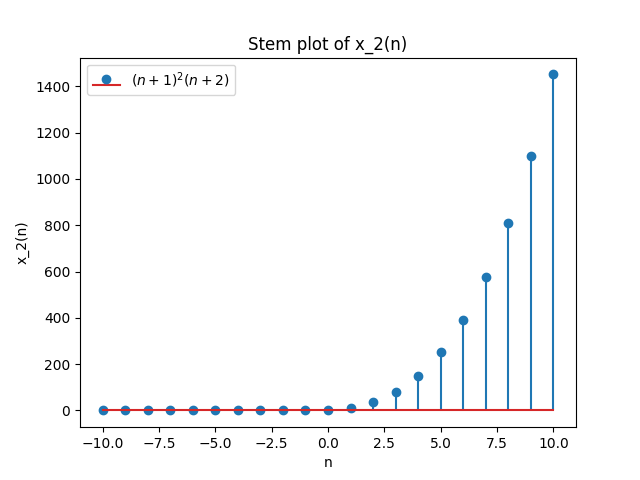
\includegraphics[width=1\columnwidth]{x2_plot.png}
    \caption{Stem Plot of $x_2\brak{n}$}
    \label{fig:x2}
\end{figure}

\begin{figure}[htbp]
    \centering
    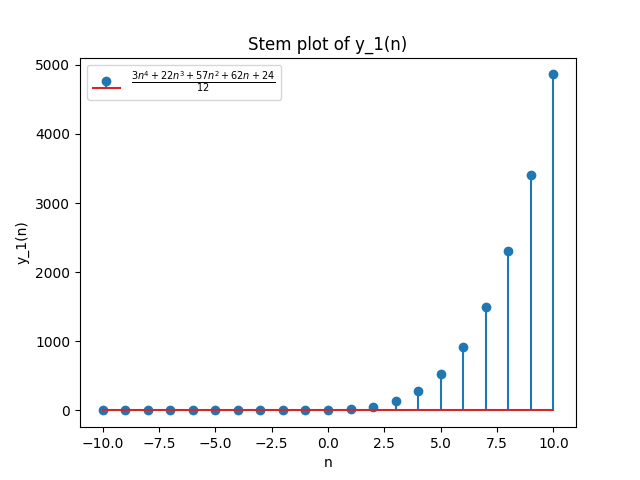
\includegraphics[width=1\columnwidth]{y1_plot.png}
    \caption{Stem Plot of $y_1\brak{n}$}
    \label{fig:y1}
\end{figure}

\begin{figure}[htbp]
    \centering
    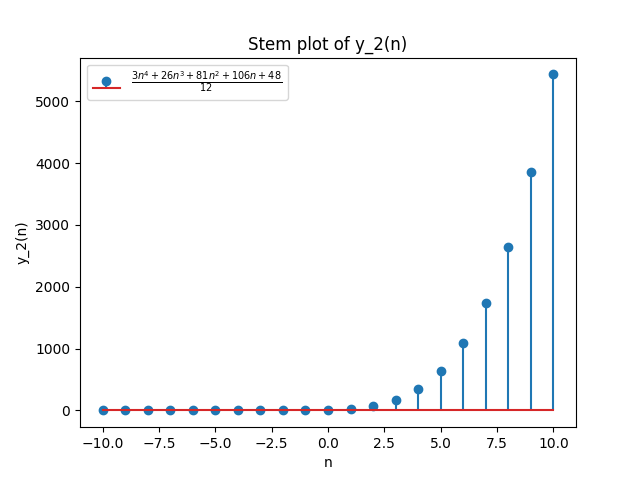
\includegraphics[width=1\columnwidth]{y2_plot.png}
    \caption{Stem Plot of $y_2\brak{n}$}
    \label{fig:y2}
\end{figure}
\end{document}
